\documentclass[aspectratio=169]{beamer}

\usepackage[czech]{babel}
\usepackage[utf8]{inputenc}
\usepackage[T1]{fontenc}
\usepackage{csquotes}
\usepackage{soul}
\usepackage{booktabs}
\usetheme[
  workplace=fi,
]{MU}

\title[MTB v4]{Návrh a implementace nového protokolu sběrnice MTBbus}
\subtitle[Obhajoba]{Obhajoba diplomové práce}
\author[J. Horáček]{Jan Horáček\texorpdfstring{\\}{, }horacekj@mail.muni.cz}
\institute[FI MU]{Fakulta informatiky Masarykovy univerzity}
\date{\today}
\subject{Návrh a implementace nového protokolu sběrnice MTBbus}
\keywords{mtb,mtbbus,stm32,avr,arm,pcb,rs485,protokol}
\begin{document}

\begin{frame}[plain]
\maketitle
\end{frame}

\section{Kontext}
\subsection{PLC}

%------------------------------------------------

\begin{frame}{Kontext: Programmable Logic Controller}
\begin{columns}
	\begin{column}{.6\textwidth}
		\begin{itemize}
		\item Základní jednotka průmyslové automatizace.
		\item Čte vstupy, nastavuje výstupy.
			\begin{itemize}
			\item Koncové snímače, motory, lasery apod.
		\end{itemize}
		\item Komunikuje s dalšími PLC obvody, s počítačem.
		\item RTOS, robustní.
		\item Řízení dopravních křižovatek, výrobních linek, elektráren apod.
		\item V této práci: nemá vlastní inteligenci.
		\begin{itemize}
		\item \textbf{PLC tvoří rozhraní mezi hardwarem a počítačem.}
		\end{itemize}
		\end{itemize}
	\end{column}
	\begin{column}{.4\textwidth}
		\begin{figure}
		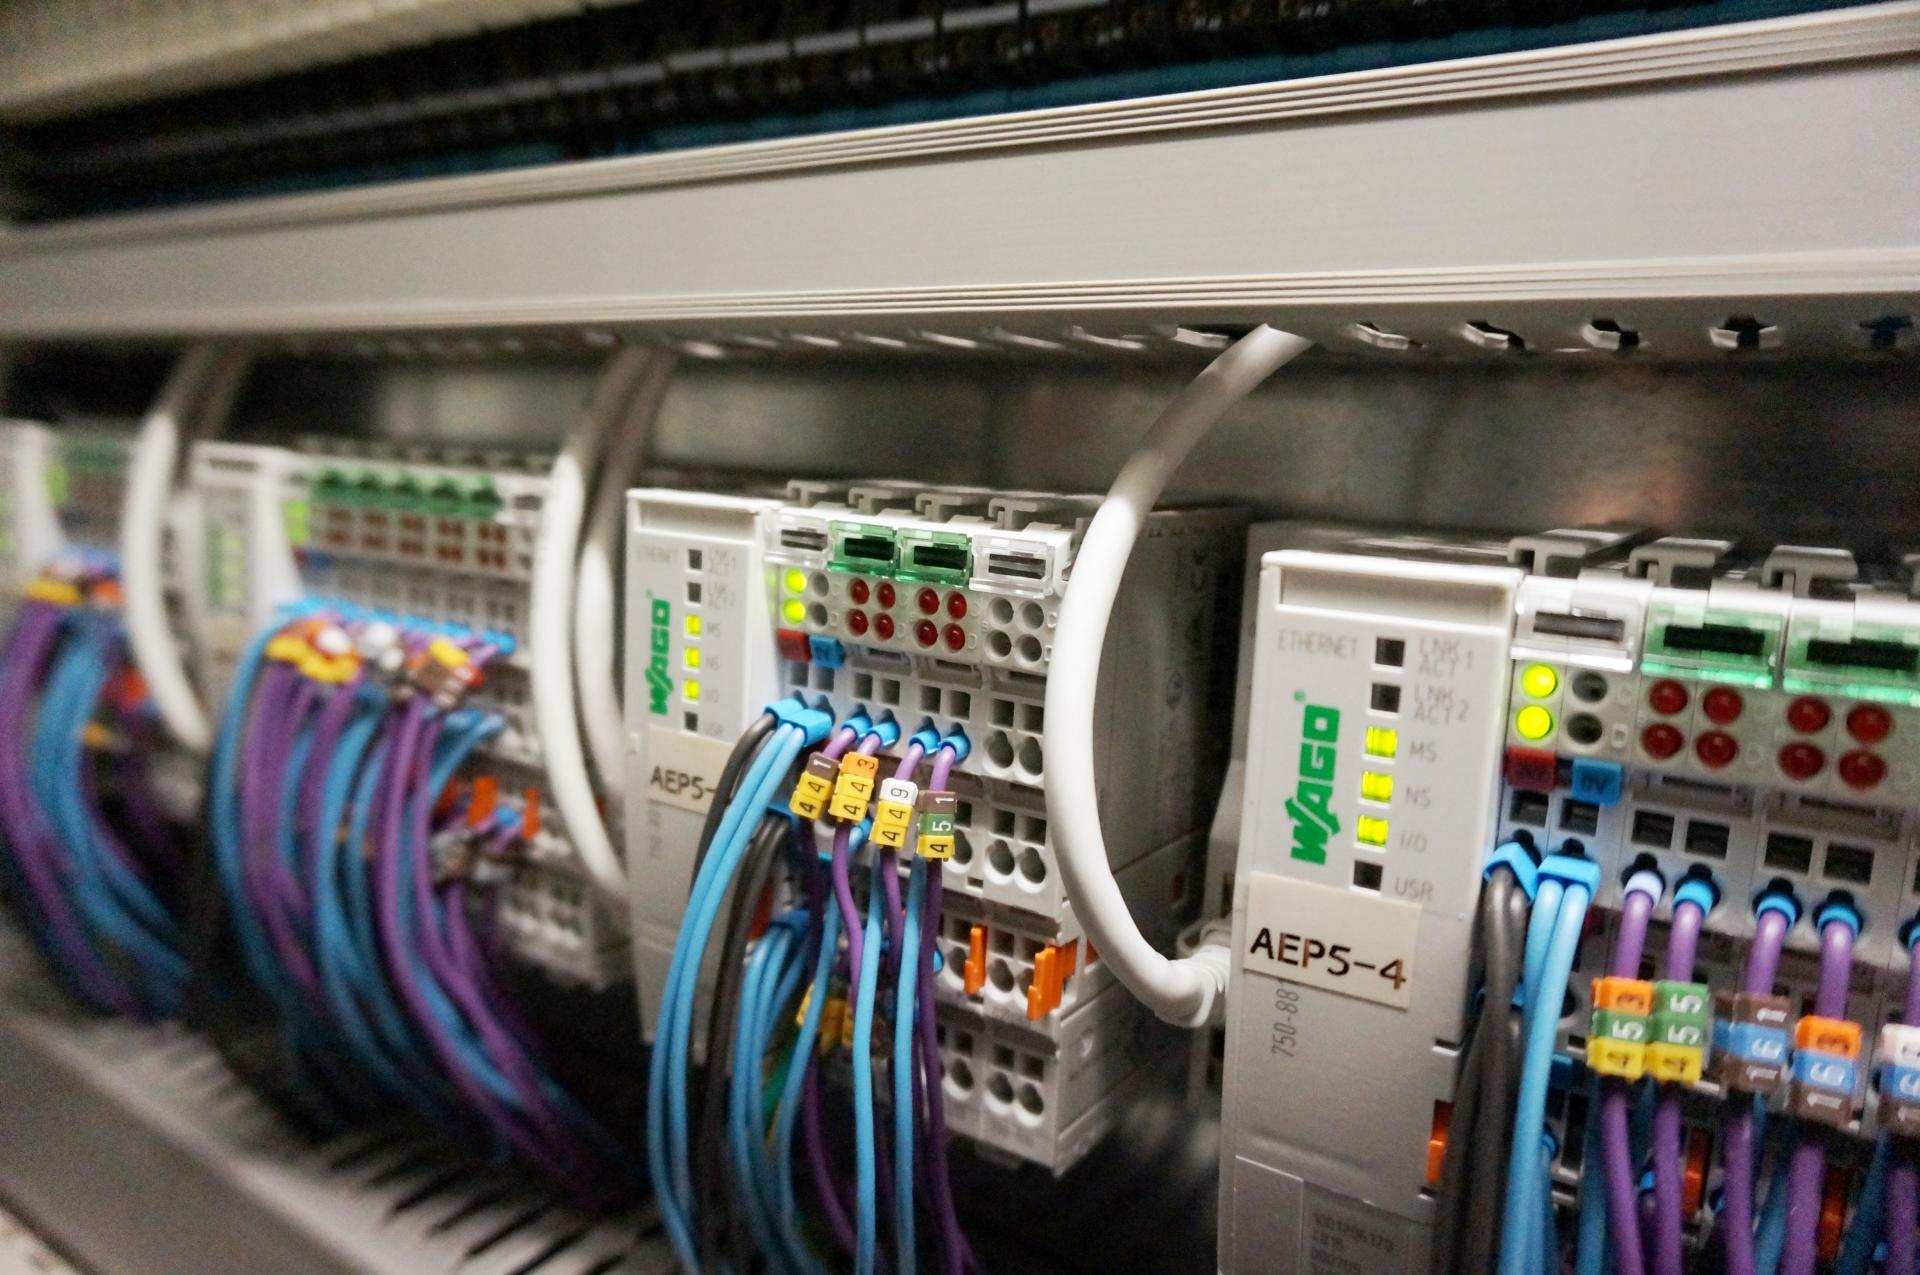
\includegraphics[width=\columnwidth]{data/plc.jpg}
		\caption{Ukázka PLC modulů.}
		\end{figure}
	\end{column}
\end{columns}
\end{frame}

%------------------------------------------------

\subsection{Řízeni modelových kolejišť}

\begin{frame}{Kontext: PLC v řízení modelového kolejiště}
\begin{figure}
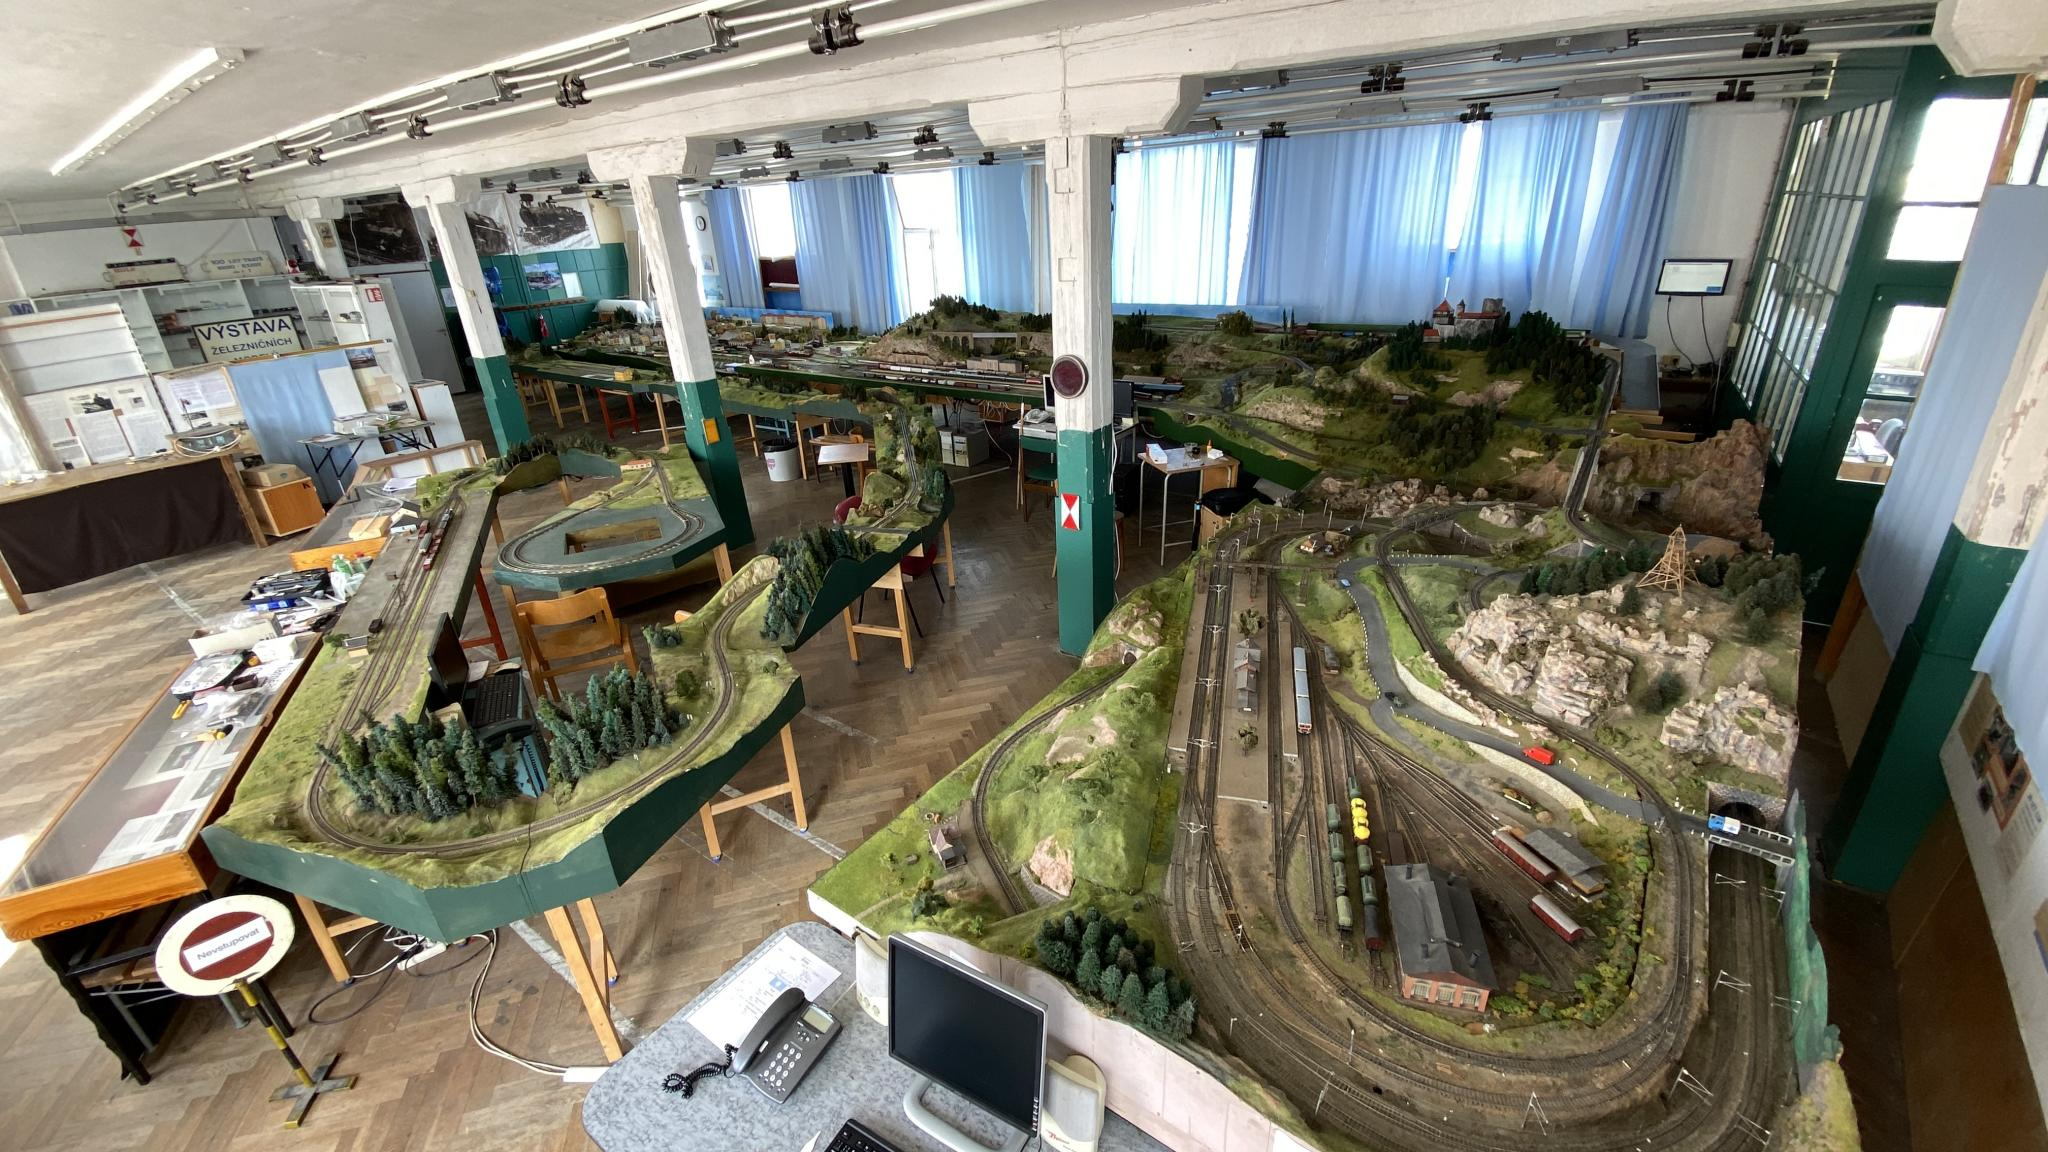
\includegraphics[width=0.8\columnwidth]{data/kolejisteMosilana.jpg}
\end{figure}
\end{frame}

%------------------------------------------------

\begin{frame}{Kontext: PLC v řízení modelového kolejiště}
\begin{columns}
	\begin{column}{.3\textwidth}
		\begin{itemize}
		\item 13 stanic.
		\item 186 výhybek.
		\item 306 úseků.
		\item 233 návěstidel.
		\item 13 přejezdů.
		\item 100 rozpojovačů.
		\item \textbf{70 MTB modulů.}
		\end{itemize}
	\end{column}
	\begin{column}{.65\textwidth}
		\begin{figure}
		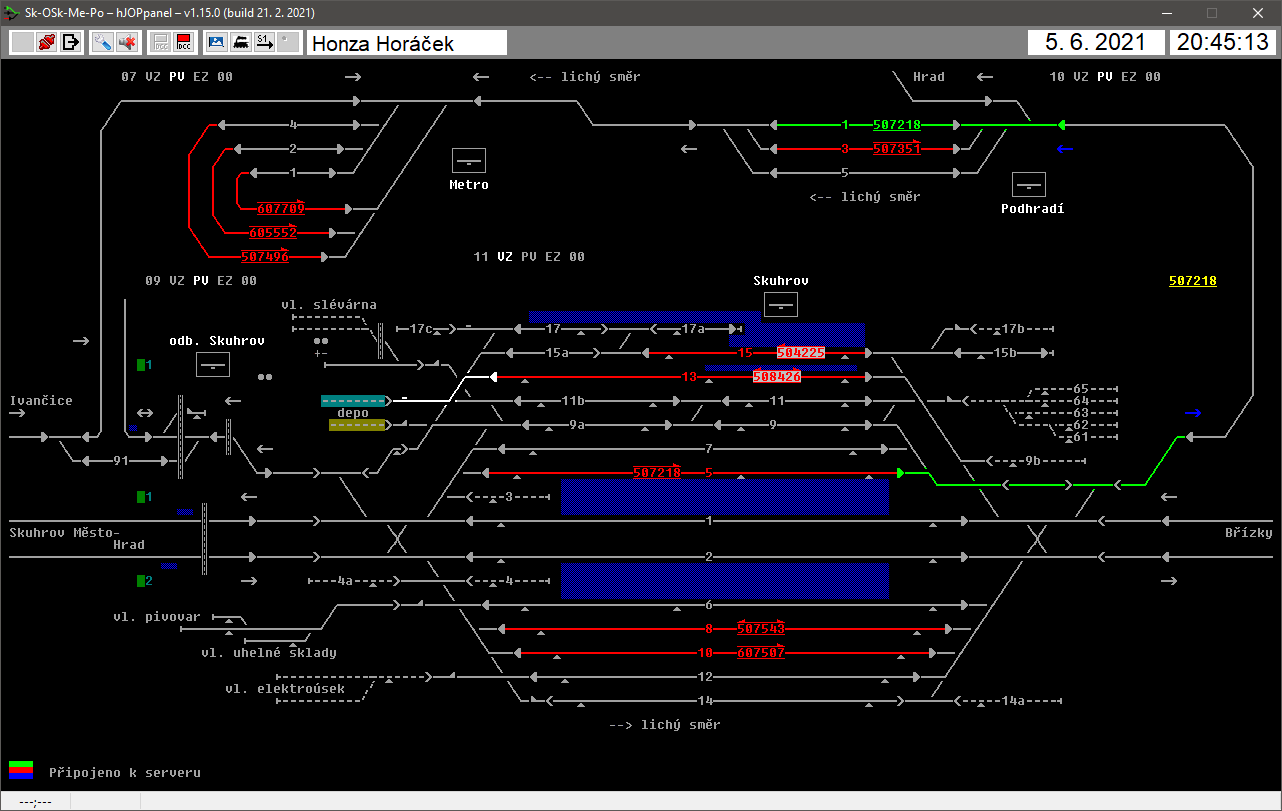
\includegraphics[width=\columnwidth]{data/sk.png}
		\caption{Ukázka řídicího rozhraní kolejiště.}
		\end{figure}
	\end{column}
\end{columns}
\end{frame}

%------------------------------------------------

\begin{frame}{Systém MTB a jeho současné nasazení}
\begin{columns}
	\begin{column}{.6\textwidth}
		\begin{itemize}
		\item Vlastní systém vyvinutý okolo roku 2000.
		\item 1 kolejiště = 1 sběrnice MTBbus.
		\begin{itemize}
			\item 1 MTB-USB modul, více \textit{MTB modulů}.
		\end{itemize}
		\item \textit{Master-slave} topologie.
		\item Různé MTB moduly:
		\begin{enumerate}
			\item MTB-UNI, MTB-UNIm,
			\item MTB-TTL,
			\item MTB-REG,
			\item MTB-POT.
		\end{enumerate}
		\item Používá se pouze pro řízení \textit{příslušenství}, nikoliv
		pro řízení jízdy.
		\end{itemize}
	\end{column}
	\begin{column}{.4\textwidth}
		\begin{figure}
		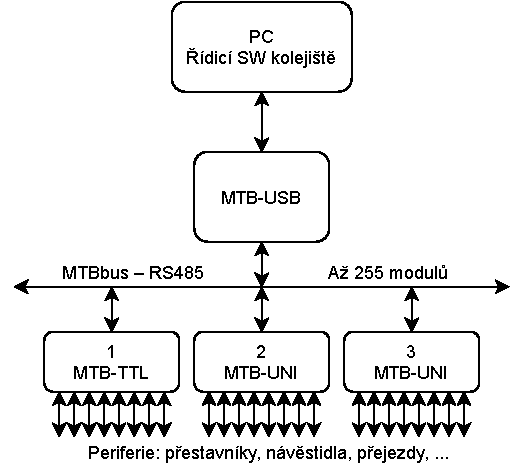
\includegraphics[width=\columnwidth]{data/mtb-topology.pdf}
		\caption{Topologie systému MTB v2.}
		\end{figure}
	\end{column}
\end{columns}
\end{frame}

%------------------------------------------------

\begin{frame}{Problémy systému MTB (v KMŽ Brno I)}
\begin{enumerate}
\item Chybí výrobní data.
\item Licenční spory.
\item Zastaralý hardware.
\begin{itemize}
\item Nemožnost aktualizovat software.
\item Některé součástky se nevyrábí.
\end{itemize}
\end{enumerate}
\pause
\begin{alertblock}{Důsledky}
Nemožnost rozšiřovat kolejiště, omezená udržitelnost, nemožnost rozvoje systému.
\end{alertblock}
\pause
\begin{alertblock}{Závěr}
Je třeba přejít na nový systém.
\end{alertblock}
\end{frame}

%------------------------------------------------

\section{Návrh MTB v4}
\subsection{Požadavky}

\begin{frame}{Požadavky na MTB v4}
\begin{enumerate}
\item MTB-UNI – umožnit kmitavé výstupy.
\item MTB-UNI – umožnit S-COM výstupy na všech výstupních pinech.
\item Univerzální návrh pro různé typy modulů (i do budoucna).
\item Vyřešit zpětnou kompatibilitu se stávajícími moduly.
\item Přístup skrze \textit{hJOP RCS API}.
\item Více možných řídicích SW v počítači.
\item Hot-swap MTB modulů, detekce nefunkčních.
\item Identifikační LED.
\item Aktualizace FW MTB modulů po MTBbus.
\item Využít komponenty s dlouhodobou dostupností.
\item Opensource \& openhardware.
\end{enumerate}
\end{frame}

%------------------------------------------------

\subsection{Návrh}

\begin{frame}{Návrh MTB v4}
\begin{columns}
	\begin{column}{.3\textwidth}
		V rámci práce vznikl:
		\begin{enumerate}
		\item nový protokol MTBbus,
		\item MTB-USB v4,
		\item MTB-UNI v4,
		\item MTB-2-AVR,
		\item IRdet,
		\item MTB Daemon,
		\item hJOP MTB RCS Network Library.
		\end{enumerate}
	\end{column}
	\begin{column}{.4\textwidth}
		\begin{figure}
		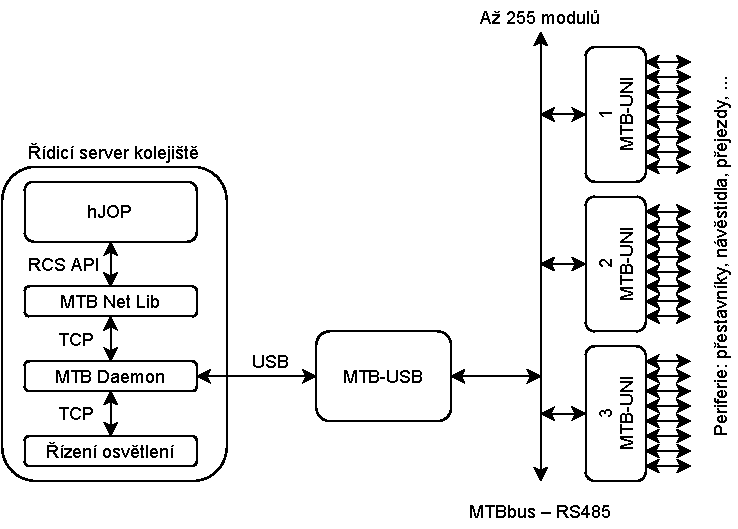
\includegraphics[width=\columnwidth]{data/new-topology.pdf}
		\caption{Topologie systému MTB v4.}
		\end{figure}
	\end{column}
	\begin{column}{.3\textwidth}
		\begin{figure}
		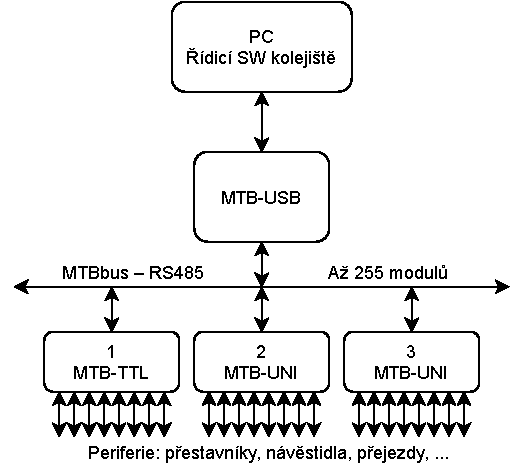
\includegraphics[width=\columnwidth]{data/mtb-topology.pdf}
		\caption{Topologie systému MTB v2.}
		\end{figure}
	\end{column}
\end{columns}
\end{frame}

%------------------------------------------------

\subsection{MTBbus}

\begin{frame}{MTBbus v4}
\begin{columns}
	\begin{column}{.5\textwidth}
		\begin{itemize}
		\item Hardware sběrnice zachován: RS485.
		\item Protokol navrhnut od základů znovu.
		\begin{itemize}
			\item Rychlost zachována: $38\ 400$ – $115\ 200$ Bd
			\item Zachováno využití devitibitové komunikace.
			\item Zachován princip \textit{master-slave}.
		\end{itemize}
		\item Modul musí vždy odpovědět na každou zprávu.
		\end{itemize}
	\end{column}
	\pause
	\begin{column}{.5\textwidth}\texttt{\footnotesize
> Module 1 Inquiry \\
< Acknowledgement  \# Modul 1 žije, \\
  žádná data k odeslání \\
> Module 2 Inquiry \\
\# Timeout – modul 2 nežije \\
> Module 3 Inquiry \\
< State of inputs changed, \\
  new state: 0b00001010 0b11110000 \\
> Module 6 Inquiry \\
< Acknowledgement \\
> Set Outputs of module 1 to\\
  0b00101010 0b01000101 \\
< Outputs Set to 0b00101010 0b01000101 \\
> Module 10 Inquiry \\
< Acknowledgement \\
...}
	\end{column}
\end{columns}
\end{frame}

%------------------------------------------------

\begin{frame}{MTBbus v4}{Zpráva}
Každá \textit{zpráva} se skládá z devítibitových slov.
\begin{enumerate}
\item Adresa modulu (jen ve směru master $\rightarrow$ slave).
\item Délka zprávy.
\item Kód zprávy.
\item Data zprávy (až 120 bytů).
\item Kontrolní součet CRC-16 (2 byty).
\end{enumerate}

\begin{exampleblock}{Příklad zprávy: \texttt{0x105 0x001 0x001 0x0D0 0x051}}
\begin{enumerate}
\item \texttt{0x105}: zpráva pro modul s~adresou 5.
\item \texttt{0x001}: následuje 1 byte zprávy.
\item \texttt{0x001}: kód zprávy \texttt{0x01}.
\item \texttt{0x0D0}, \texttt{0x051}: kontrolní součet \textit{CRC-16}.
\end{enumerate}
\end{exampleblock}
\end{frame}

%------------------------------------------------

\begin{frame}{MTBbus v4}{Typy zpráv, dvouvrstvost zpráv}
\footnotesize
\begin{columns}
	\begin{column}{.45\textwidth}
		\texttt{0x01} \textit{Module Inquiry} \\
		\texttt{0x02} \textit{Module Information Request} \\
		\texttt{0x03} \textit{Set Configuration} \\
		\texttt{0x04} \textit{Get Configuration} \\
		\texttt{0x05} \textit{Beacon} \\
		\texttt{0x10} \textit{Get Input} \\
		\texttt{0x11} \textit{Set Output} \\
		\texttt{0x12} \textit{Reset Outputs} \\
		\texttt{0x20} \textit{Change Address} \\
		\texttt{0xE0} \textit{Change Speed} \\
		\texttt{0xF0} \textit{Firmware Upgrade Request} \\
		\texttt{0xF1} \textit{Firmware Write Flash} \\
		\texttt{0xF2} \textit{Firmware Write Flash Status Request} \\
		\texttt{0xFE} \textit{Module-specific Command} \\
		\texttt{0xFF} \textit{Reboot}
	\end{column}
	\begin{column}{.45\textwidth}
		\texttt{0x01} \textit{Acknowledgement} \\
		\texttt{0x02} \textit{Error} \\
		\texttt{0x03} \textit{Module Information} \\
		\texttt{0x04} \textit{Module Configuration} \\
		\texttt{0x10} \textit{Input Changed} \\
		\texttt{0x11} \textit{Input State} \\
		\texttt{0x12} \textit{Output Set} \\
		\texttt{0xF2} \textit{Firmware Write Flash Status} \\
		\texttt{0xFE} \textit{Module-specific Command}
	\end{column}
\end{columns}
\end{frame}

%------------------------------------------------

\section{Nový hardware}
\subsection{MTB-USB v4}

\begin{frame}{MTB-USB v4}
\begin{columns}
	\begin{column}{.4\textwidth}
		\begin{figure}
		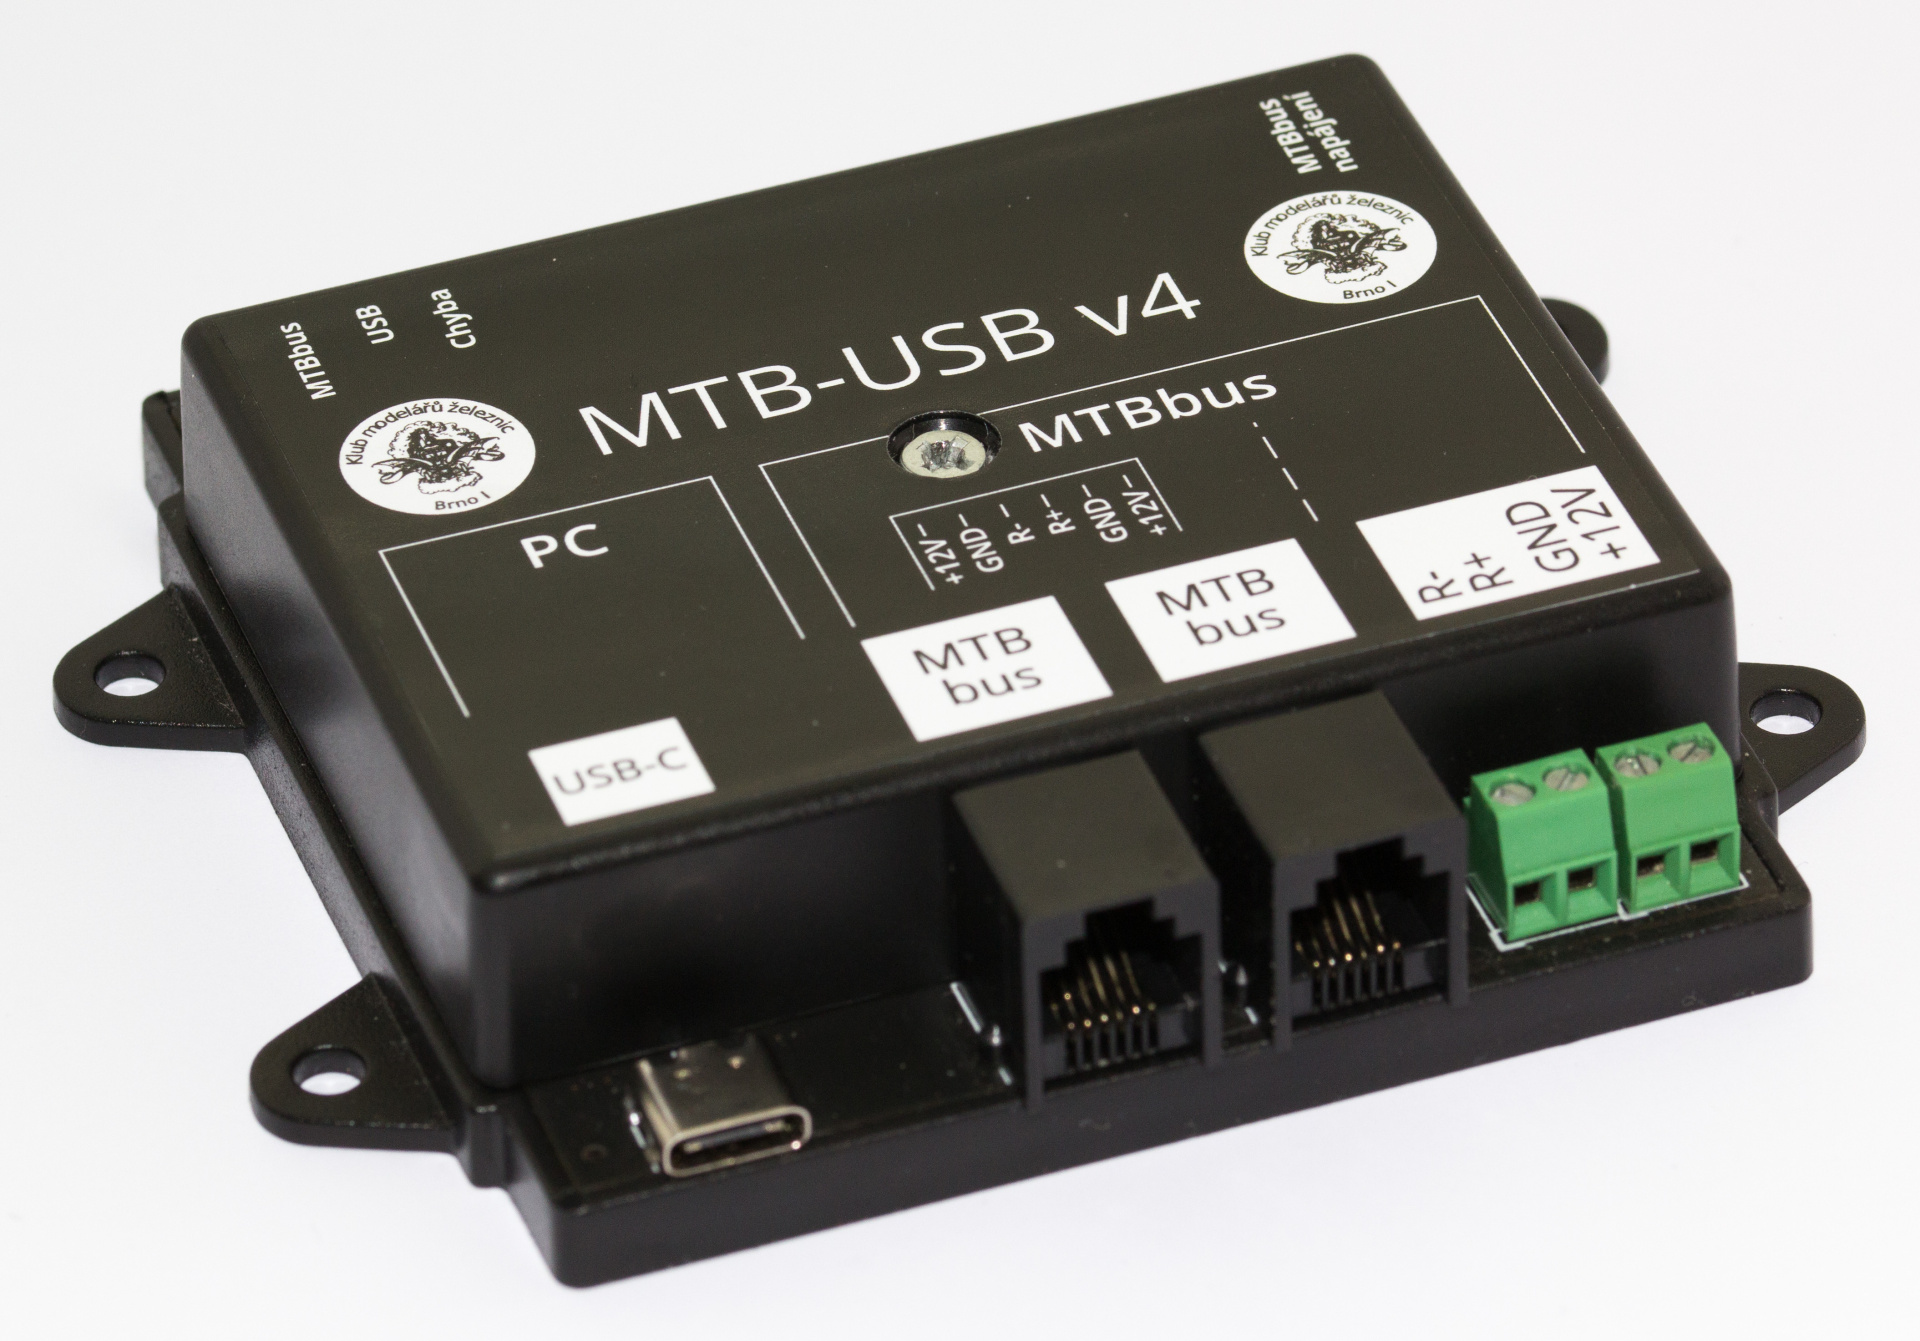
\includegraphics[width=\columnwidth]{data/usb-all.jpg}
		\end{figure}
	\end{column}
	\begin{column}{.6\textwidth}
		\begin{figure}
		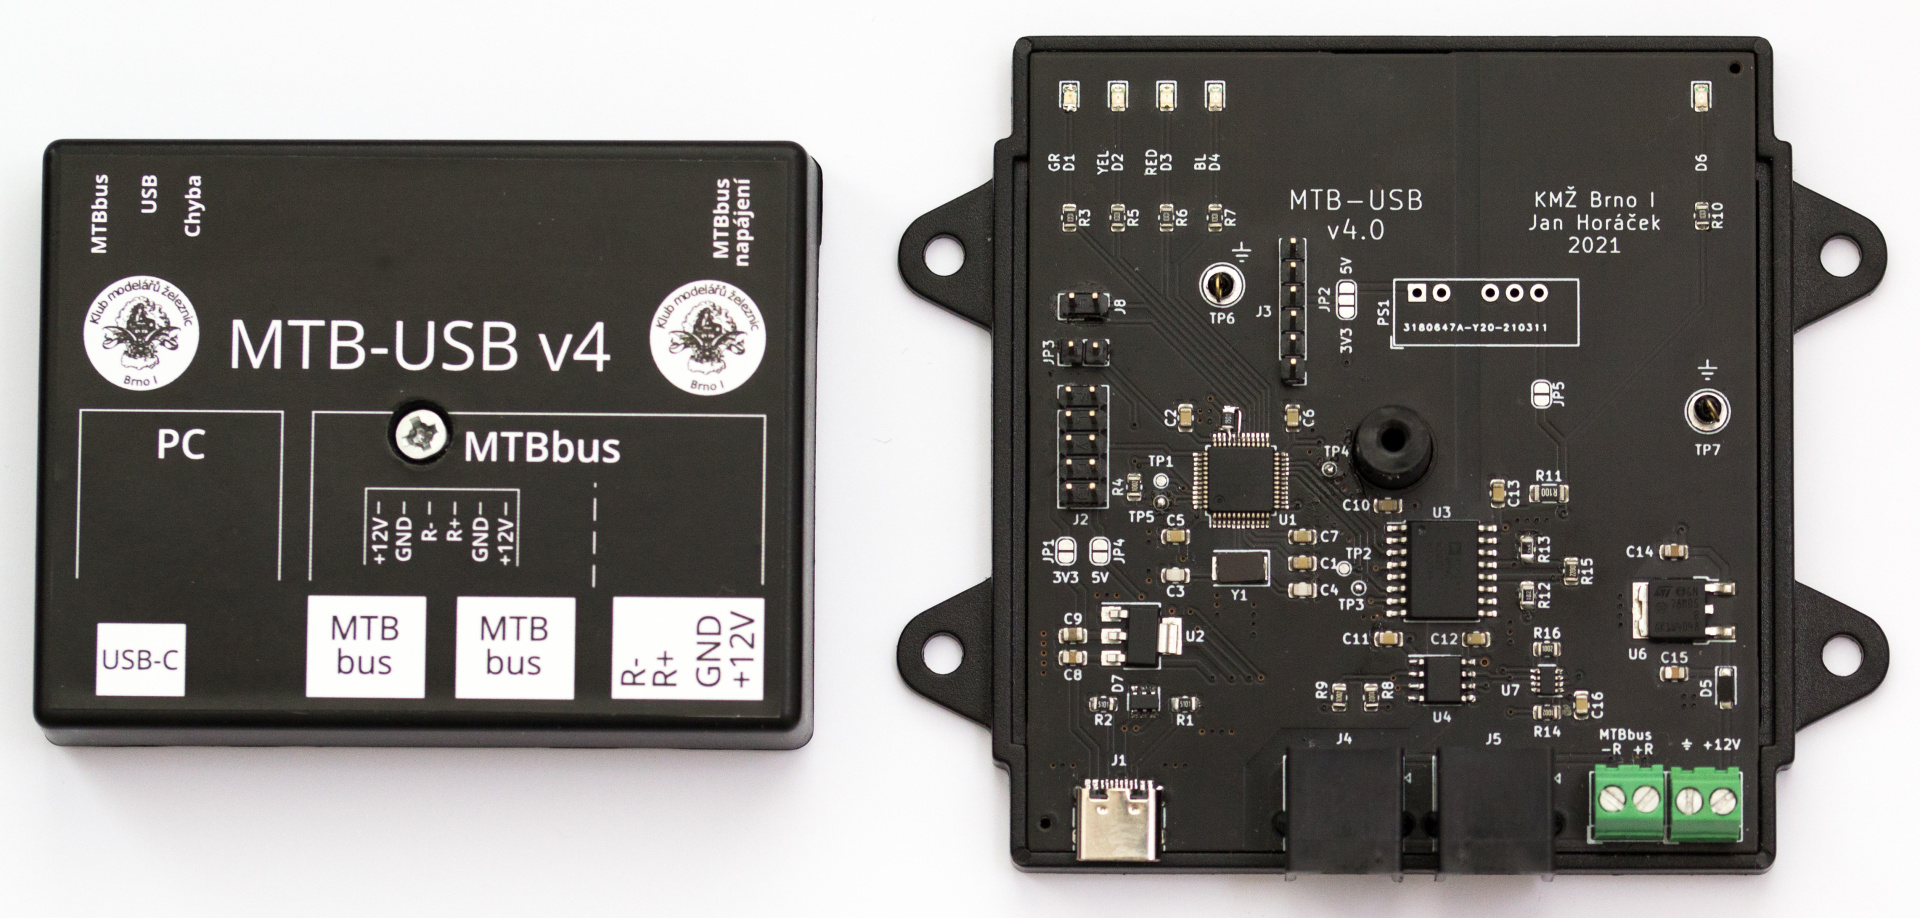
\includegraphics[width=\columnwidth]{data/usb-inside.jpg}
		\end{figure}
	\end{column}
\end{columns}
\end{frame}

%------------------------------------------------

\begin{frame}{MTB-USB v4}
\begin{enumerate}
\item Přeposílá data mezi MTBbus a počítačem.
\item Záměrně neobsahuje složitou logiku.
\item Vykonává časově kritické operace sběrnice MTBbus.
\item Provádí \textit{polling} modulů.
\item Udržuje seznam aktivních modulů.
\item Provádí retransmise zpráv do MTBbus při nedoručení.
\end{enumerate}
\end{frame}

%------------------------------------------------

\begin{frame}{Komunikační protokol s počítačem}
\begin{itemize}
\item Nejdůležitější příkaz: \textit{Forward Packet}.
\item Počítač může vyžádat seznam aktivních modulů.
\item MTB-USB posílá počítači asynchronně události na sběrnici.
\item Detailní popis protokolu v textu práce.
\end{itemize}

\begin{alertblock}{Zpráva}
Uvozena speciální sekvencí bytů \texttt{0x2A} \texttt{0x42}.
\end{alertblock}
\end{frame}

%------------------------------------------------

\begin{frame}{Hardware}
\begin{itemize}
\item USB a MTBbus část desky galvanicky oddělené.
\begin{itemize}
\item Napájení USB části z USB-C.
\item Napájení MTBbus části: přes měnič nebo externí napájení.
\end{itemize}
\item Procesor \texttt{STM32F103}.
\begin{itemize}
\item Přímá podpora USB.
\item V USB části DPS.
\end{itemize}
\item Budič RS485 \texttt{ADM2483}.
\item Automatické osazování na \textit{JLCPCB}.
\item KiCad.
\end{itemize}
\end{frame}

%------------------------------------------------

\begin{frame}{Firmware}
\begin{itemize}
\item C
\item STM32 HAL
\item DMA
\end{itemize}
\end{frame}

%------------------------------------------------

\subsection{MTB-UNI v4}

\begin{frame}{MTB-UNI v4}
\begin{columns}
	\begin{column}{.5\textwidth}
		\begin{itemize}
		\item 16 digitálních vstupů.
		\item 16 digitálních výstupů.
		\item Napájení 7–17 V DC.
		\item Adresování pomocí jumperů.
		\item Procesor ATmega128.
		\begin{itemize}
			\item Hlavní program a bootloader.
		\end{itemize}
		\end{itemize}
	\end{column}
	\begin{column}{.5\textwidth}
		\begin{figure}
		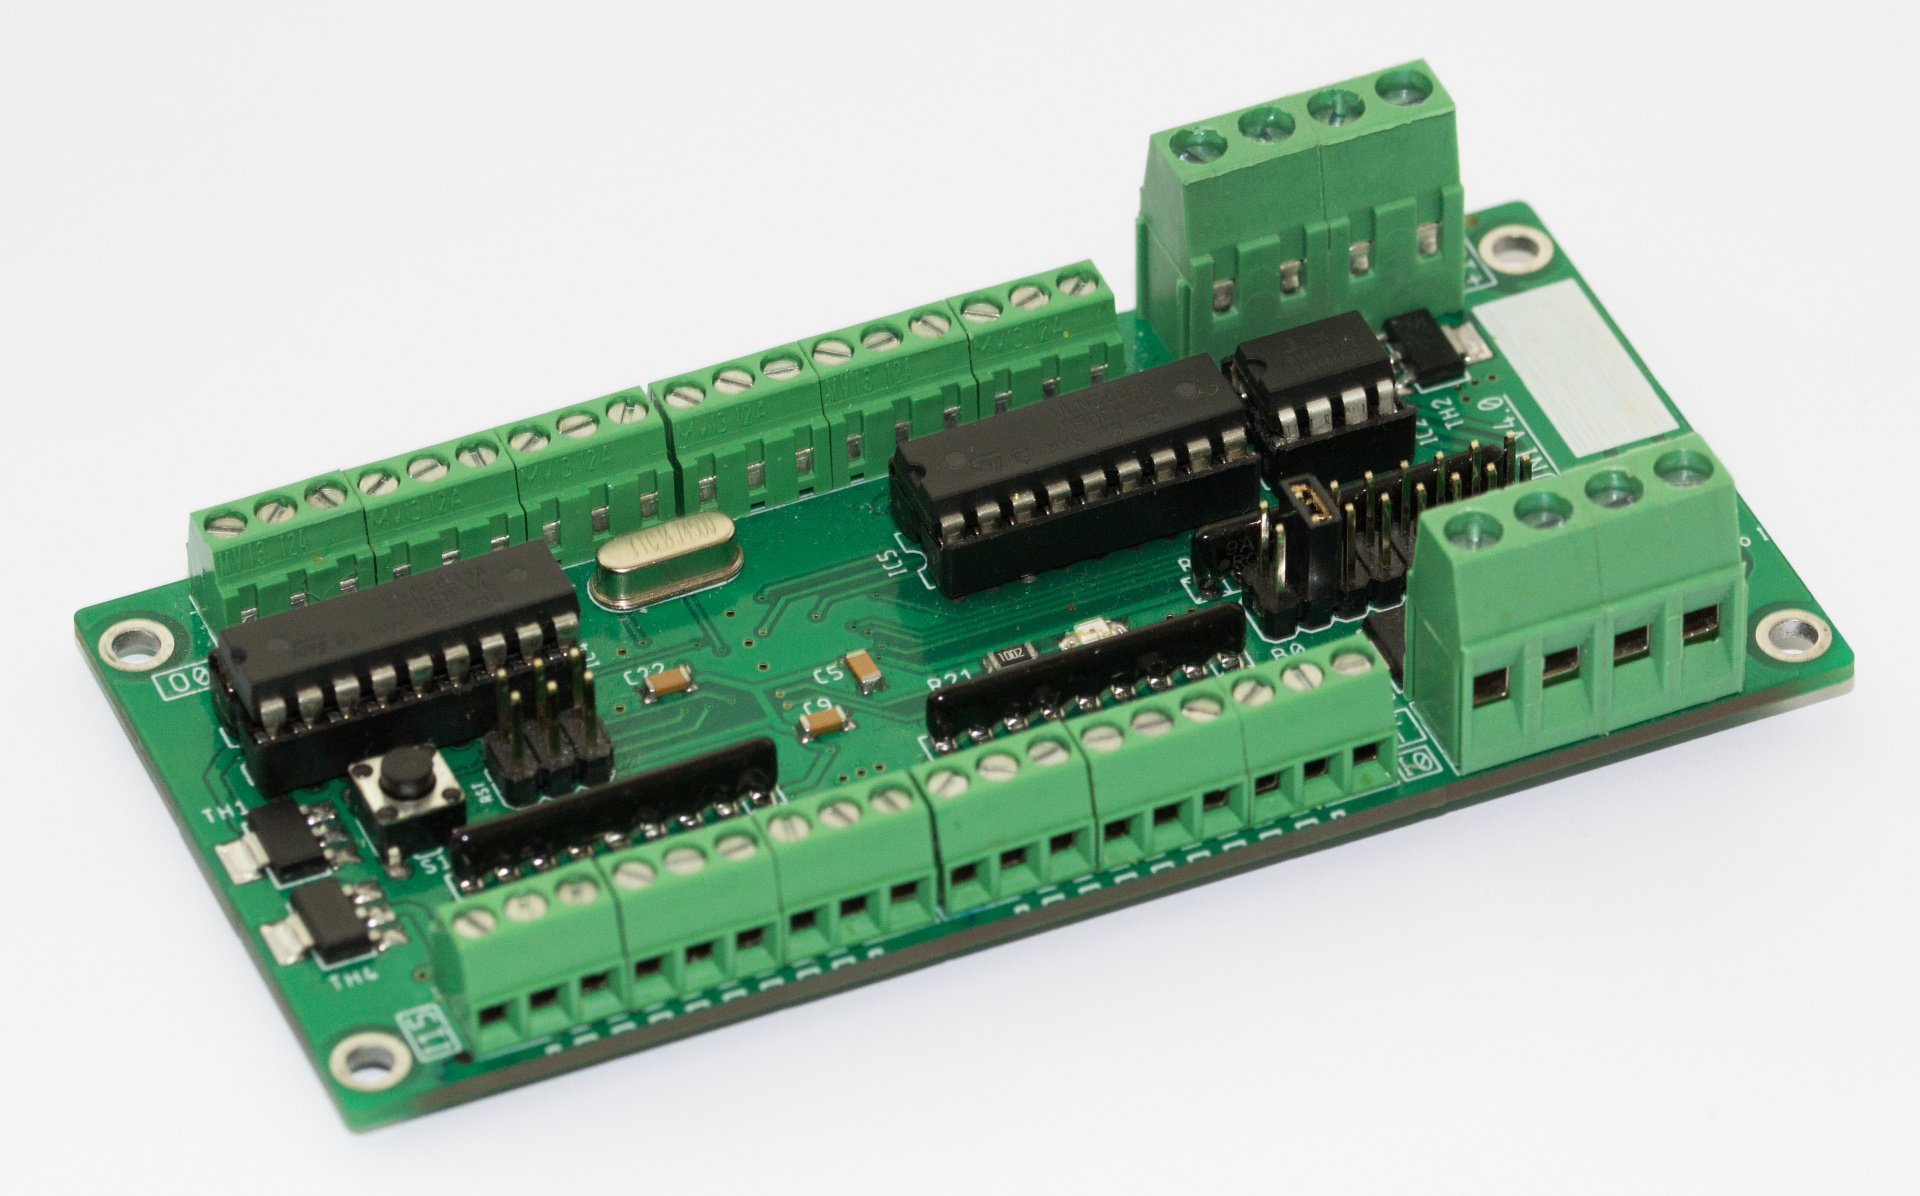
\includegraphics[width=\columnwidth]{data/uni-v40-screw-all.jpg}
		\caption{Ukázka modulu MTB-UNI v4.}
		\end{figure}
	\end{column}
\end{columns}
\end{frame}

%------------------------------------------------

\subsection{MTB-2-AVR}

\begin{frame}{MTB-2-AVR}
\begin{columns}
	\begin{column}{.5\textwidth}
		\begin{itemize}
		\item Použije se místo procesoru v původních MTB modulech.
		\item Univerzální deska pro MTB-UNI, MTB-UNIm a MTB-TTL.
		\item Upgrade sběrnice na v4 nevyžaduje nákladnou výměnu modulů.
		\item Procesor ATmega328p.
		\begin{itemize}
			\item Hlavní program a bootloader.
		\end{itemize}
		\end{itemize}
	\end{column}
	\begin{column}{.5\textwidth}
		\begin{figure}
		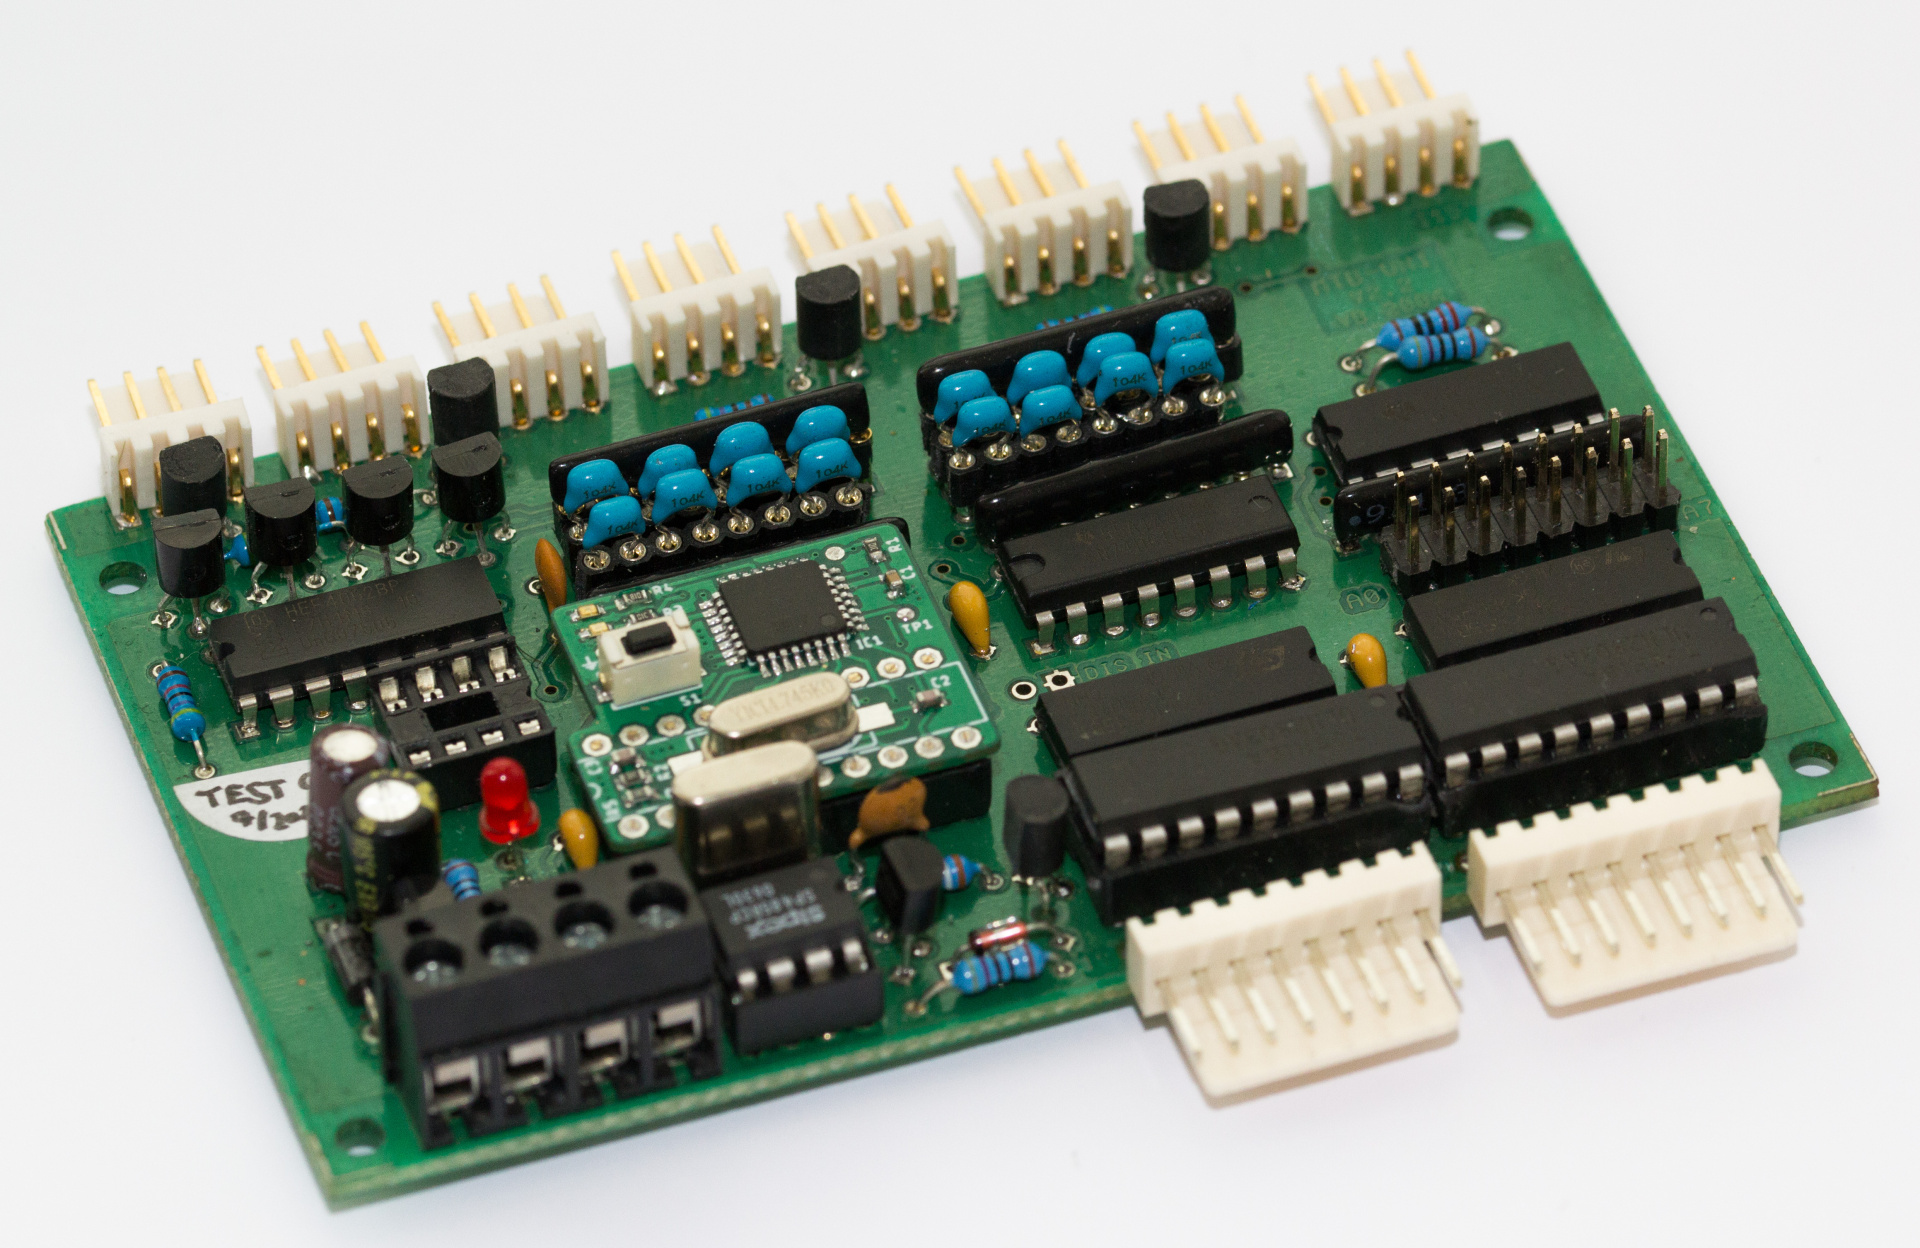
\includegraphics[width=\columnwidth]{data/uni-2-upgrade-all.jpg}
		\caption{Nástavná deska MTB-2-AVR v modulu MTB-UNI v2.}
		\end{figure}
	\end{column}
\end{columns}
\end{frame}

%------------------------------------------------

\subsection{IRdet}

\begin{frame}{IRdet}
\begin{columns}
	\begin{column}{.7\textwidth}
		\begin{itemize}
		\item Nahrazuje přímou podporu IR čidel v původních MTB-UNI.
		\item Není připojena na MTBbus.
		\item 8 IR čidel.
		\item 8 digitálních opticky oddělených výstupů.
		\item Univerzální.
		\end{itemize}
	\end{column}
	\begin{column}{.3\textwidth}
		\begin{figure}
		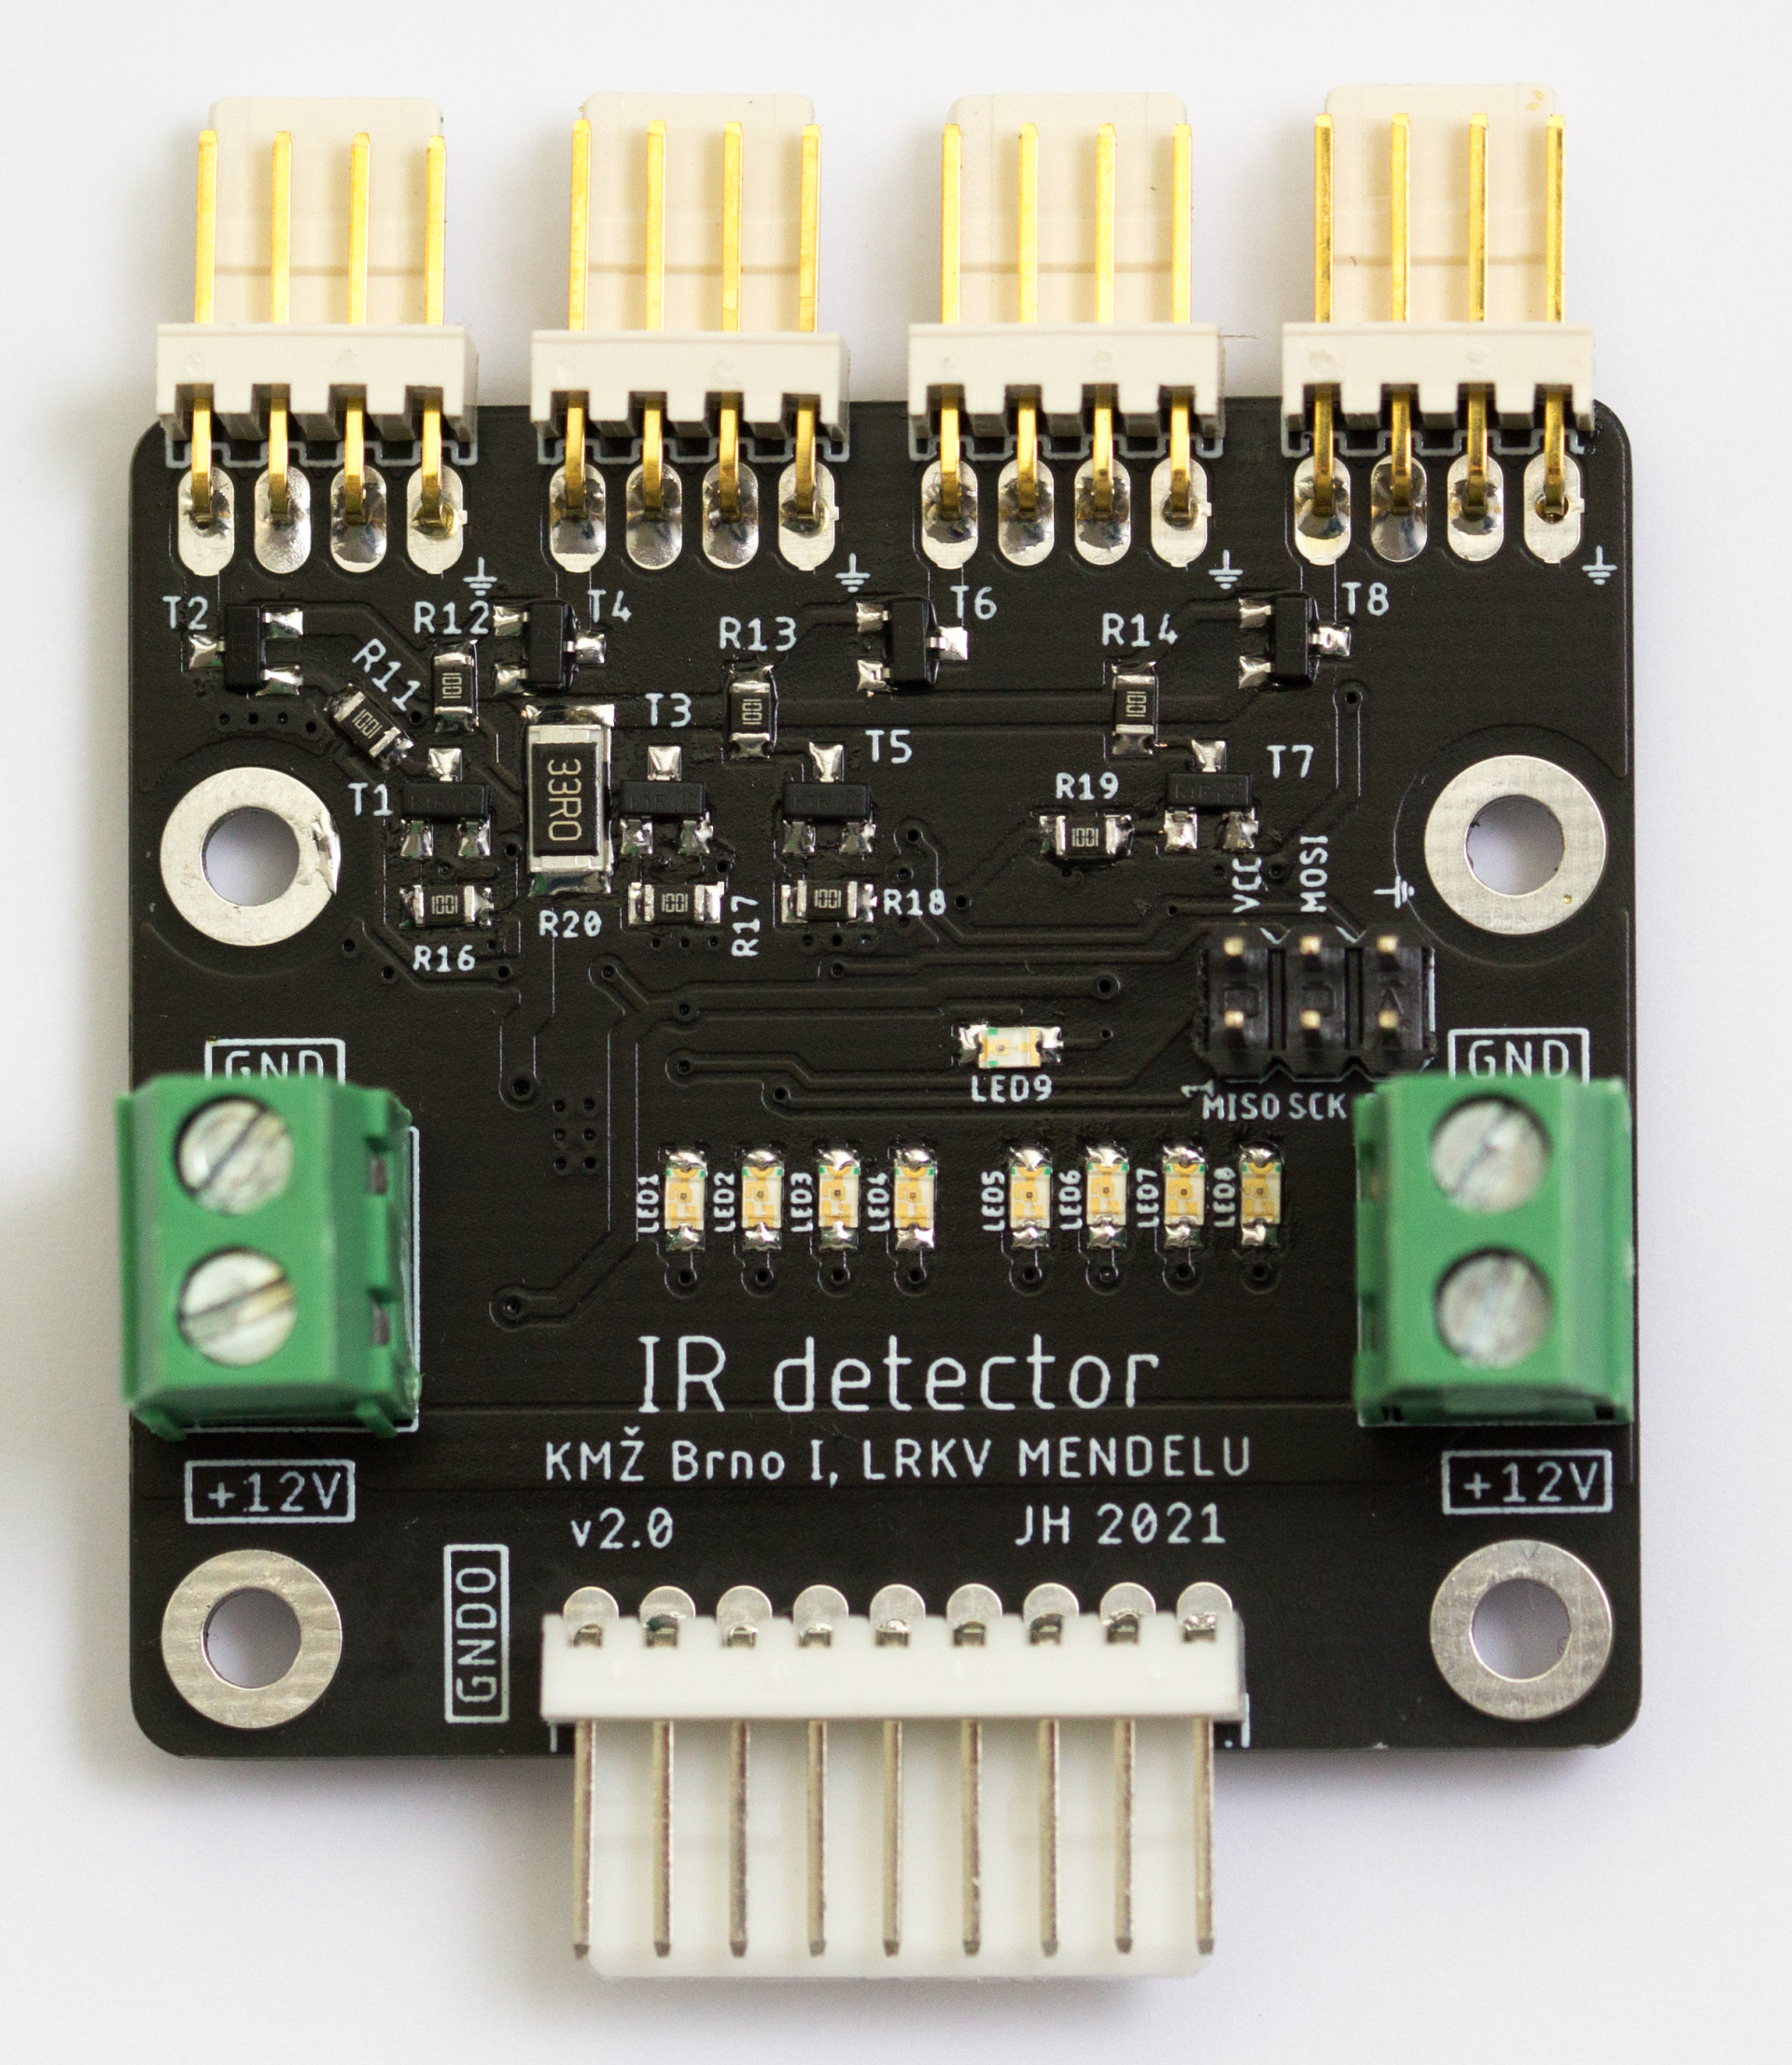
\includegraphics[width=\columnwidth]{data/irdet-front.jpg}
		\caption{Deska IRdet.}
		\end{figure}
	\end{column}
\end{columns}
\end{frame}

%------------------------------------------------

\section{Nový software}
\subsection{MTB Daemon}

\begin{frame}{MTB Daemon}
\begin{columns}
	\begin{column}{.5\textwidth}
		\begin{itemize}
			\item Umožňuje připojení více řídicích SW k MTB.
			\item Udržuje konfiguraci modulů.
			\item Poskytuje \textit{hezké} API.
		\end{itemize}
		Implementace:
		\begin{itemize}
			\item JSON TCP Server.
			\item USB CDC.
			\item C++.
			\item Qt.
			\item Multiplatformní.
		\end{itemize}
	\end{column}
	\begin{column}{.5\textwidth}
		\begin{figure}
		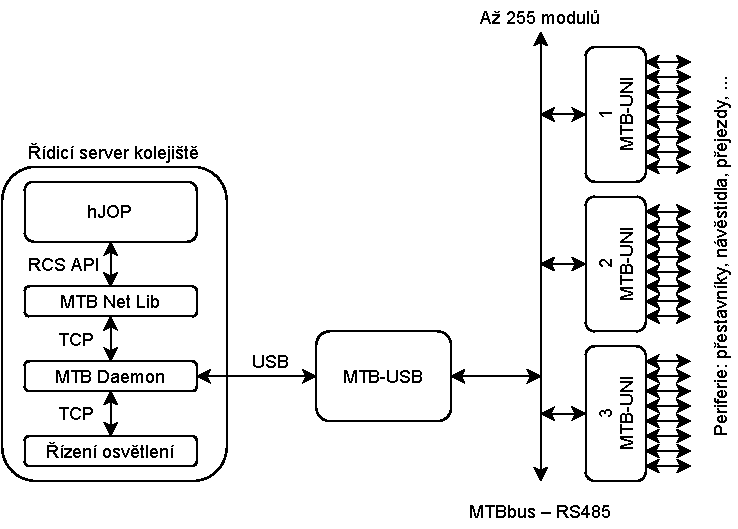
\includegraphics[width=\columnwidth]{data/new-topology.pdf}
		\caption{Topologie systému MTB v4.}
		\end{figure}
	\end{column}
\end{columns}
\end{frame}

%------------------------------------------------

\subsection{hJOP MTB Network Library}

\begin{frame}{hJOP MTB Network Library}
\begin{columns}
	\begin{column}{.5\textwidth}
		\begin{itemize}
			\item Integruje MTB v4 do aktuálně nasazeného SW \textit{hJOP} pro
			řízení kolejišť v KMŽ Brno I.
		\end{itemize}
		Implementace:
		\begin{itemize}
			\item C++.
			\item Qt.
			\item Dll.
			\item Windows.
		\end{itemize}
	\end{column}
	\begin{column}{.5\textwidth}
		\begin{figure}
		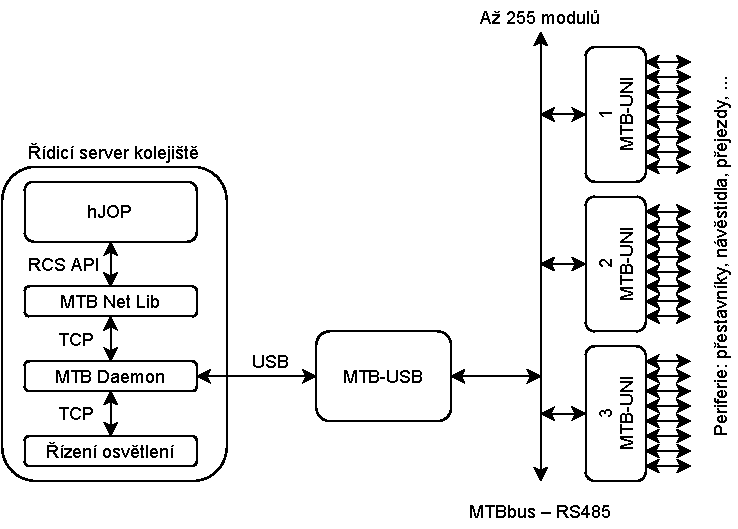
\includegraphics[width=\columnwidth]{data/new-topology.pdf}
		\caption{Topologie systému MTB v4.}
		\end{figure}
	\end{column}
\end{columns}
\end{frame}

%------------------------------------------------

\section{Závěr}

\begin{frame}{Závěr}
\begin{columns}
	\begin{column}{.5\textwidth}
		V rámci práce vznikl:
		\begin{enumerate}
		\item nový protokol MTBbus,
		\item MTB-USB v4,
		\item MTB-UNI v4,
		\item MTB-2-AVR,
		\item IRdet,
		\item MTB Daemon,
		\item hJOP MTB RCS Network Library.
		\end{enumerate}
	\end{column}
	\begin{column}{.5\textwidth}
		\begin{figure}
		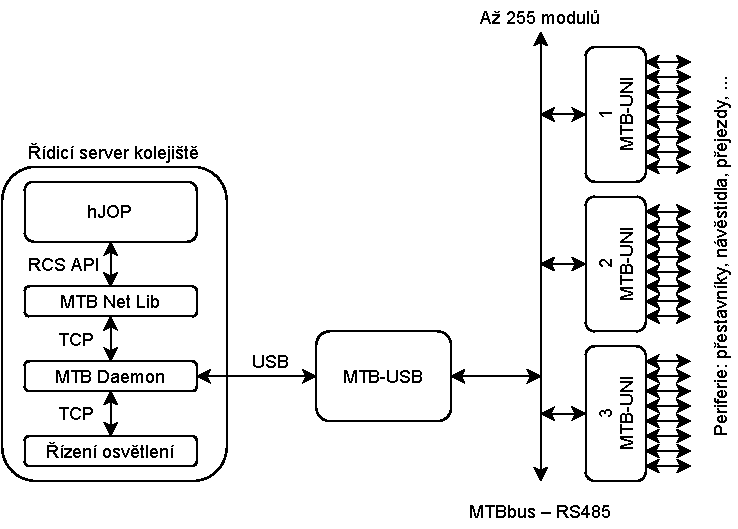
\includegraphics[width=\columnwidth]{data/new-topology.pdf}
		\caption{Topologie systému MTB v4.}
		\end{figure}
	\end{column}
\end{columns}
\end{frame}

%------------------------------------------------

\begin{frame}{Nasazení}
\begin{itemize}
\item Květen 2021: menší stanice o 4 MTB modulech.
\item Červen 2021: jedno klubovní kolejiště o 20 MTB modulech.
\item Výhled červenec 2021: největší klubovní kolejiště o 70 MTB modulech.
\end{itemize}
\end{frame}

%------------------------------------------------

\begin{frame}{Přínos}
\begin{enumerate}
	\item Vznikl otevřený a spolehlivý systém pro řízení příslušenství modelových
		kolejišť, který může využít kdokoliv.
	\item Rozšíření bezpečného řízení modelové železnice.
	\item Zpřístupnění řízení kolejiště méně pokročilým programátorům.
	\item Možnost využití pro řízení jiných systémů než modelových kolejišť.
\end{enumerate}

\begin{alertblock}{Přínos pro KMŽ Brno I}
\begin{enumerate}
\item Umožněno zprovoznění řízení silniční a tramvajové dopravy.
\item Umožněno řízení osvětlení.
\item Umožněno nasazení pultů obsluhy.
\item Umožněno vytvoření nových zesilovačů a RailCom modulů s cílem nasazení
	na lokomotivní depo. Otevřena cesta k vyšší spolehlivosti kolejiště.
\item Umožněna optimalizace výstupů MTB-UNI modulů.
\item Umožněna snazší diagnostika.
\end{enumerate}
\end{alertblock}
\end{frame}

\begin{frame}{Možná rozšíření}
\begin{enumerate}
\item Další typy MTB modulů.
\item Podpora MTB v komerčních SW pro řízení kolejišť.
\item Vyšší rychlosti sběrnice.
\item Automatická detekce rychlosti sběrnice.
\end{enumerate}
\end{frame}

%------------------------------------------------

\end{document}
